
%this sets up the defaults for the documents, 12pt font and A4 size. The article type sets this up as such as opposed to letter or memo.

%for the finer points LaTeX see https://en.wikibooks.org/wiki/LaTeX or http://tex.stackexchange.com/

\documentclass[12pt,a4paper]{article}
\usepackage{titlesec} 
\usepackage{fancyhdr}
 \usepackage[pagebackref,hidelinks]{hyperref}
\usepackage[hypcap]{caption}
\usepackage[utf8]{inputenc}
\usepackage{graphicx} 
\usepackage[parfill]{parskip} 
\usepackage{lscape}
%%% PACKAGES
\usepackage{booktabs} % for much better looking tables
\usepackage{array} % for better arrays (eg matrices) in maths
\usepackage{paralist} % very flexible & customisable lists (eg. enumerate/itemize, etc.)
\usepackage{verbatim} % adds environment for commenting out blocks of text & for better verbatim
\usepackage{subfig} % make it possible to include more than one captioned figure/table in a single float
\usepackage[toc,page]{appendix}
% These packages are all incorporated in the memoir class to one degree or another...
\usepackage{xcolor}
\colorlet{GREEN}{green}
\colorlet{RED}{red}
\colorlet{BLUE}{blue}
%header and footer settings
\pagestyle{fancyplain}
\fancyhf{}
\renewcommand{\headrulewidth}{0.5pt}
\renewcommand{\footrulewidth}{0.5pt}
\setlength{\headheight}{15pt}
\fancyhead[L]{Neil Notman - 40124066}
\fancyhead[R]{SOC10101 Honours Project}
\fancyfoot[L]{Games Development BSc (Hons)}
\fancyfoot[C]{\thepage}
\setlength\parindent{0cm}
%set better section layout
\makeatletter
\renewcommand\subsection{\@startsection {subsection}{1}{2mm} % name, level, indent
                               {3pt plus 2pt minus 1pt} % before skip
                               {3pt plus 0pt} % after skip
                               {\normalfont\bfseries}}
\makeatother
\makeatletter
\renewcommand\section{\@startsection {section}{1}{0mm} % name, level, indent
                               {4pt plus 2pt minus 1pt} % before skip
                               {4pt plus 0pt} % after skip
                               {\bfseries}}
\makeatother

\usepackage{titlesec}
\usepackage{geometry}
\geometry{
	verbose,
	tmargin=2.5cm,
	bmargin=2.5cm,
	lmargin=3.2cm,
	rmargin=2.5cm
}
\setcounter{secnumdepth}{4}

\titleformat{\paragraph}
{\normalfont\normalsize\bfseries}{\theparagraph}{1em}{}
\titlespacing*{\paragraph}
{0pt}{3.25ex plus 1ex minus .2ex}{1.5ex plus .2ex}


\hypersetup{
	colorlinks=true,
	citecolor=GREEN,
	linkcolor=RED,
	urlcolor=BLUE}

\renewenvironment{abstract}
  {\small\quotation
  {\bfseries\noindent{\large\abstractname\\\noindent{}}}}
  {\endquotation}

\begin{document}
%you can import other documents into your main one, these layout the Title and Declarations on its own page.
%you might need to change these to \ if your on Microsoft Windows.
\newcommand{\HRule}{\rule{\linewidth}{0.5mm}}

\begin{titlepage}
	\begin{center}

	\HRule \\[0.4cm]
    	{\Large \bfseries Procedural Level Generation and Dynamic Path-finding A Combined Approach \par}
	\vspace{0.2cm}
	\HRule \\[1.5cm]

	
    	\vspace{3cm}
	\begin{minipage}{0.4\textwidth}
	\begin{center} \large
        \emph{}\\
        	Neil Notman - 40124066
			Supervisor: Dr Benjamin Kenwright\\
			Second Marker: Dr Neil Urquhart
   	 \end{center}
    	\end{minipage}
	
	\vspace{2cm}
    	\begin{minipage}{1\textwidth}
    	\begin{center} \large

		Submitted in partial fulfilment of \\
		the requirements of Edinburgh Napier University \\
		for the Degree of \\
        BSc Games Development (Hons) 
    	\end{center}
    	\end{minipage}

    	\vfill

    	% Bottom of the page
	\begin{minipage}{1\textwidth}
    	\begin{center} \large
		School of Computing
    	\end{center}
    	\end{minipage}
	
	\vspace{1cm}
    	{\large \today}


	\end{center}
\end{titlepage}


\section*{Authorship Declaration}
\vspace{0.5cm}
\begin{flushleft}
I, (Neil Notman), confirm that this dissertation and the work presented in it are my own achievement.\newline

Where I have consulted the published work of others this is always clearly attributed;\newline

Where I have quoted from the work of others the source is always given. With the exception of such quotations this dissertation is entirely my own work;\newline

I have acknowledged all main sources of help; \newline

If my research follows on from previous work or is part of a larger collaborative research project I have made clear exactly what was done by others and what I have contributed myself;\newline

I have read and understand the penalties associated with Academic Misconduct.\newline

I also confirm that I have obtained informed consent from all people I have involved in the work in this dissertation following the School's ethical guidelines.\newline
\end{flushleft}

\begin{flushleft} \large
\emph{Signed:} \\
\end{flushleft}

\vspace{.5cm}

\begin{flushleft} \large
\emph{Date:} \\
\end{flushleft}

\vspace{.5cm}

\begin{flushleft} \large
\emph{Matriculation no: }  \\
\end{flushleft}
\pagebreak

\section*{Data Protection Declaration}
\vspace{0.5cm}
\begin{flushleft}
Under the 1998 Data Protection Act, The University cannot disclose your grade to an unauthorised person. However, other students benefit from studying dissertations that have their grades attached. \newline

\vspace{0.5cm}

Please sign your name below one of the options below to state your preference.\newline
\vspace{0.5cm}

The University may make this dissertation, with indicative grade, available to others.\newline
\vspace{3cm}


The University may make this dissertation available to others, but the grade may not be disclosed.\newline
\vspace{3cm}


The University may not make this dissertation available to others.\newline
\end{flushleft}


\pagebreak
\begin{abstract}
As games evolve and expand with the times there is an increased demand placed upon the hardware of games consoles and personal computers in terms of storage space and memory usage. This project will analyse the approaches currently available and will examine the viability of developing a combined approach to level generation and path finding with the aim of producing a solution that will compete with current approaches in terms of the quality of the terrain generated tested through the results given by the path finding and the distances between nodes that will be placed in sane (flat, reachable) locations on the terrain this will also allow for testing the quality of the path finding approach by testing against different complexities of terrain and existing industry techniques.     
\end{abstract}
\pagebreak


\tableofcontents 
\newpage

\listoftables

\newpage

\listoffigures

\newpage

\section*{Acknowledgements}
\subsection*{}

\newpage
\section{Introduction}

\subsection{Procedural Level Generation}
Procedural level generation is the process of creating a level through an algorithm contained within a computer program instead of using software to create this content then loading it into a program. The procedural level generation approach was mainly utilised in the early day of games development where storage space was a major concern.\\The first game to contain procedurally generated levels was Richard Garriott's  game Akalabeth: World of Doom which was published by California Pacific Computer Company in 1980 \cite{Akalabeth}.\\\\This project is going to utilise procedural level generation to create a average sized game world by creating a height-map which is a grey-scale image then reading the data from a height-map and using this data to transform a plane to create a large scale landscape in chunks.

\subsection{Path-Finding}
Path-Finding is an area of Artificial Intelligence that allows for definition what parts of a given level can be moved to by computer controlled players this is done by creating a set of nodes on walkable areas then linking these nodes together to form a path there are various algorithms that accomplish this task. A time-line of path-finding developments is given at figure: \ref{timeline}. The project will attempt to use path-finding on the generated level in small chunks to allow for faster processing and access to more optimisation techniques.  
\subsection{Optimisation Techniques}
There are many factors that can affect the run-time performance of computer programs and a similar amount of approaches that can be utilised to improve performance some of the most prominent techniques in this area include use of multi-threading and parallelism frameworks such as OpenMP for use in single computer based solutions and MPI which allows for parallel implementation over a network.

There are other options that differ from a parallel approach that could be utilised these can include memory alignment of instructions or a graphics processing unit (GPU) based implementation.      

\subsection{Aims and Objectives}
\label{Aims}
The main aim of this project is to examine and test the viability of combining level generation and path finding algorithms to create a double ended testing mechanism for quality to allow a performance based assessment between both level of detail in the terrain when compared with the time taken for a path finding technique to find a correct path.\\\\
   The aim of this project will be achieved by completion of the following objectives which include both design and implementation as shown below.
   
   \subsubsection{Design objective}
   The main design objective will be the creation of a graphical user interface that provides a suitable visualisation of the implemented solution and displays all relevant data. There are various libraries that allow for and assist with the creation of such interfaces such as GLFW for Opengl based applications however the windows SDK also contains this ability and will allow for clear differentiation from the interface and any graphical code included in the application.  
   
   \subsubsection{Implementation Objectives}
    The creation of an application using the chosen solution to allow a user to create various sizes of level.\\\\ The application will then build the terrain and perform path finding on a set of nodes positioned across the generated terrain and assess the quality of both the level and path finding technique taking into account the complexity of a given level such as obstacles slopes and caves.\\\\The application will then assess how easy it is to build a path round that level and will give a score based on both the complexity of a generated level and the path-finding technique used.\\ 


\subsection{Report Layout}
The report goes on to give a review of various literature sources associated with the project Next there will be an analysis into the methodology used in implementation and finally the testing and results will be given alongside a conclusion to the project which will discuss the overall success and knowledge gained based on the results of testing.
\newpage
\section{Literature-Review}

\setlength\parindent{0cm}

\subsection{Background and inspiration}
The inspiration for this project was based around pushing performance and analysing both level generation and path-finding approaches to find a common area where these methods can be combined to improve run-time performance and to allow testing of the quality of both the terrain and path that is built in terms of complexity against the amount of nodes required to build a logical path and any deviations that are made to the path due to constraints posed by the terrain. 

For a background of various path-finding techniques please refer to paper\cite{Time} 
\subsection{Procedural Level generation Techniques}
There are a variety of ways to generate either 2d or 3d geometry within a program this section will discuss the documented methods and compare them in terms of usability and performance.

The paper \cite{LG-Survey} examines the different layers of a game that can be procedurally generated this includes a section on game space for levels or maps and defines these both abstract or concrete methods for generation of both indoor and outdoor environments as well the paper gives a taxonomy of commonly used procedural content generation techniques.  


\subsubsection{The Diamond-Square algorithm}
This method of level generation was proposed by \cite{DSA2} is based off fractal subdivision to generate randomised terrain based on two steps which are split into the diamond step  and the square step hence the algorithms name. The diamond step of this algorithm uses the edge points of a square to generate a random value in the midpoint then the square step of this algorithm performs the same function however uses the edge points of the diamond made previously which gives a square as the result. The algorithm is recursive meaning that it performs multiple passes through each step with the generated surface gaining detail every pass however the increase in detail is due to an increase in geometry each pass this means the algorithm can be memory intensive due to the size of array to store the height values being a power of two + 1 this means for eight passes through the algorithm the array would need up to 256KB memory if storing floating point values \cite{LevelDSA}.

\subsubsection{The marching cubes algorithm}
 

\subsubsection{Height-map generation and Rendering}
A height map is a grey scale image that makes use of depth to create a section of terrain with areas where the terrain is raised being shown as brighter and lower areas shown as dark for most height maps digital noise is used to produce a suitable terrain for an example of the output of a height map please refer to figure \ref{noise}. 

\subsubsection{Perlin Noise}
\label{Perlin}
To create the image \ref{noise} Perlin Noise was used this is a gradient based noise developed by Ken Perlin in 1983 \cite{perlin} to create procedural textures using the algorithm outlined below. 
\begin{itemize}
\item Get an input point of the image 
\item Loop through the neighbours of this point
\item Generate a pseudo-random gradient vector.
\begin{figure}[h]
\centering
\item perform the following calculation
\begin{equation}
\label{eq:Noise}
G \cdot(P-Q)
\end{equation}
\caption{G= gradient vector P = input point Q = Neighbouring point}
\label{noise:eq}
\end{figure}

This equation will give the value of P where G is equal to 0 at point Q.
\item Finally you Interpolate between the the points down to your point, using an S-shaped cross-fade curve e.g( 
\begin{math}(eg: 3t^2-2t^3)\end{math}) this will give the weighting applied in each dimension.This step will require computing of the curve n times, followed by 2n-1 linear interpolations to get the final result.
\end{itemize}

\subsection{Path-finding Techniques}
This section will address some of the key path finding techniques that would address the problem posed within the project an analysis of past work done in this area will be given with the aim to analyse how this can be utilised and expanded within the context of the project. 
\subsubsection{Dijkstra's algorithm}
The algorithm for path finding presented by Edsger Dijkstra in 1959 \cite{dijkstra} allows searching of a weighted graph to determine the shortest route through a set of nodes by working out the shortest path from one node to every other connected node in the graph this is known as a uniform cost search. The nodes can be used to represent space within either a two dimensional grid or a point in three dimensions. This method can be used within the project as the cost of travelling between nodes can be calculated as the euclidean distance between the nodes this will allow us to remain with vector calculations which would benefit a GPU based implementation. If we look at figure \ref{timeline} it is shown there have been a number of developments to this method of path-finding the main adjustments that are beneficial to the project will be discussed below.
\paragraph{Developments to graph based path finding}
There have been a multitude of developments to graph based path finding techniques these include the techniques mentioned in \ref{timeline} the main developments and their benefits in the context of this project will be discussed.

The first development to graph based techniques that is interesting is the article by \cite{goodchild} this was where the traditional orthogonal approach to building paths was modified due to the fact that errors were produced with straight line and smoothly curved paths the solution was to look at using both the orthogonal and diagonal steps to reduce the errors produced such as deviation from the path and this also prevents the path from becoming too long.

Another development of interest is the creation of a spread based algorithm for path-finding that was first proposed by \cite{califano} the origin of the splash (structural pattern localization analysis by sequential histograms) algorithm was to identify patterns in amino acids and other uses within the field of computational biology relying on sparse pattern matching techniques however the splash is shown in \cite{califano} to be both memory and computationally efficient when compared with other path finding methods that utilise sparse pattern matching this is of value as it allows for a path that has patterns will be processed faster and using the splash algorithm could be beneficial due to the parallelizable nature of that this algorithm uses to search through data.    


\subsubsection{Path finding in games}
\label{pfg}
Path finding is an area of artificial intelligence widely used in games to allow computer controlled characters to walk on the geometry that makes up a game world or level the paper by \cite{pathfinding-games} describes the method for path finding on geometry by first building a navigational mesh which describes the parts of a given world or level can be traversed or using a node based waypoint system which is traditionally based on the visibility of one node to the next which allows for traversal of the geometry there is also a breakdown of path finding techniques into directed and undirected methods with directed methods such as the A* algorithm which combines the cost based searching of nodes or a navigational mesh with a heuristic search to the goal this allows for greater efficiency over Dijkstra's algorithm.

\subsubsection{The A* algorithm}
The A* or A star path-finding algorithm was first proposed in 1968 the paper \cite{A*} this algorithm for path-finding uses a heuristic based search to find the shortest route for a given weighted graph there are many benefits to using this algorithm these include storing previously any visited nodes that do not lead to the goal this helps to prevent backtracking and eliminate infeasible solutions leading to a reduction in the search space thus an increase in runtime performance although this comes with an increased memory overhead as a result of using two lists over one list to store the path.   
\subsubsection{Analysing the quality of path-finding techniques}
\label{quality}
The niche of this project is that there has been no previous attempt to quantify the quality of procedural level development techniques with regards to ease of path-finding as a factor for the assessment of quality and assess path-finding with regards to the complexity of a terrain that is generated this will be achieved through the development of a deep learning AI system that can learn from it's own examples other systems that utilise this method of learning such as the system developed by google\textsuperscript(tm) in their deep mind department called alphago which was used to beat the current champion of the game GO\cite{AI-learning} this was made possible by training the system with the moves of experts then allowing it to learn from playing against itself using two neural networks one to determine promising moves and the other searches ahead of the promising moves found this reduces the search space allowing this processing to take place as a brute force approach would fail due to the magnitude of moves possible in this project the AI system could be utilised to fine tune the metric for level complexity by learning how to score an environment and gradually increasing the consistency of results gathered.


\subsubsection{Previous work in this field}
There has been a previous honours project based on performance of GPU based path-finding. The thesis that was authored by \cite{honours} contains work on a variety of path-finding techniques including Dijkstra, A* and diffusion methods with both a sequential and parallelised implementation the optimised versions of these path-finding approaches which may be utilised in cases of performance bottleneck as this project will not be specifically related to performance but rather the production of an elegant constrained path and suitable terrain.

\subsection{Optimisation techniques}
To optimise the project a wide range of factors and approaches are being considered the purpose and uses of these will be briefly discussed below along with a discussion on how these methods could benefit this project.\\

\subsubsection{Parallelism and parallel programming approaches}
The first approach to address is that of how to get the most performance out of the development platform (PC) one of the main ways to optimise for this platform is the use of parallel programming this will be implemented through the OpenMP API \cite{Openmp}which is built into Visual Studio this will allow for multi-threading of any code running on the central processing unit (CPU) through the use of pre-processor directives to specify sections of code to incorporate parallelism this approach should give a performance increase by utilising the multiple cores in the central processing unit over a sequential implementation that uses a single core.

Other parallel frameworks have been considered however are not at this point set to be implemented these are the MPI (Message Passing Interface)\cite{mpi} which allows for distributed parallelism over a network this would be extremely beneficial to performance as the PC that the program is running on would have more resources available however this approach can have issues mainly due to the communication being network based meaning that bandwidth can affect the performance of the program to produce a performance decrease due to these factors it is unlikely that the project will utilise this technique. 

\subsubsection{Graphics Processing Unit (GPGPU)}
GPGPU(General Purpose Graphics Processing Unit) programming allows the user to run non graphics based code on the GPU this is beneficial due to the amount of processing cores that the GPU contains over the central processing unit  however there area number of drawbacks to this approach and it can only be used within certain problem area's for example GPGPU programming is a good fit to math based problems over large data sets in comparison to problems that branch through sections of code this is due to the way data is processed on the GPU this is done by streaming the data through the GPU cores in groups known as either wavefronts or wraps which are groups of threads within the GPU and the terminology for these differs depending on the technology used instead of the normal fetch execution cycle of the CPU where instructions and resources are fetched from memory before they are executed or loaded. To utilise the GPU for processing we must send the data from the CPU to the GPU then perform our operations and finally transfer the answer from the GPU back to the CPU this is one of the main drawbacks to GPGPU programming as the performance is determined not only by the hardware but also by the speed of data transfer between the CPU and GPU and the size that this data takes up in memory.    

The use of GPGPU techniques for parallel programming were only recently applied to AI because of the branching nature of the problems in this area it has always been considered that  the AI system discussed in \ref{quality} used a distributed system to utilise the hardware resources of multiple machines to carry out parts of the processing this is what allowed the massive amount of processing power required to allow the alphago system to process the best moves at every point of a match. 

\subsection{Commercial packages}
There exist a number of commercial applications that fall within the context of this project most of these are contained within  games engines which contain ways to generate levels and to build paths and evolutionary systems which are generally used to find the best solution can be found within lots of packages one of the most noteable being journey planning software such as that contained within Google Maps. 

\pagebreak


\newpage
\section{Technical Information}
This section will look at the hardware based issues with the project and will show updates to hardware utilisation.


\newpage
\section{Implementation Methodology}
This section will analyse how the different areas of the implementation are approached and seek to explain how these approaches work at a technical level.

For a basic outline of the expected execution of the project please refer to figure \ref{block}
\subsection{Level Generation}
To generate the three dimensional terrain used in the project a height-map was generated through the use of the Libnoise external library which is discussed below.

\subsubsection{Libnoise external library}
This external library generates different types of noise as shown by figure \ref{noise} this is achieved use of various modules that can produce different types of noise including Perlin which is the basis for our output shown in \ref{heightmap} another feature of this library is that it allows the noise generated to be written out to various graphical file types for the height-map in the project a Bitmap (BMP) graphical file type was produced which is then loaded into the project and stored in a data structure for manipulation and rendering.\\
\begin{figure}[ht!]
	
\includegraphics[width=0.5\textwidth]{images/heightmaptest}
	\caption{An image showing the output image that was generated by noise}	 \label{noise}
\end{figure}

\pagebreak
When this image is rendered to the screen against a depth buffer on the GPU it gives the following output:
\begin{figure}[ht!]
	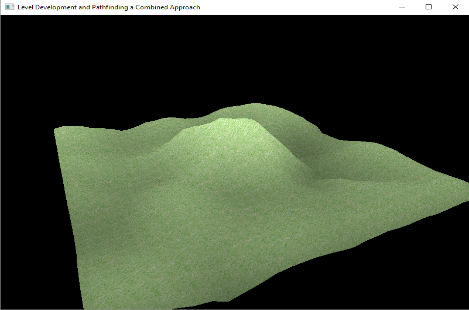
\includegraphics[width=0.5\textwidth]{images/Heightmap-output}
	\caption{The output from rendering a heightmap} \label{heightmap}
\end{figure}

\subsection{Nodes and placement} 
To place and visualise the nodes that will be utilised for any path finding technique to be used across a terrain. The glut (OpenGL Utility Toolkit) api was used to create a simple method for rendering a sphere these were then placed along the x and z axis of the terrain and position on the y-axis is checked against the height values read in from the height-map to either raise or lower the nodes to suit the terrain. 

\begin{figure}[ht!]
	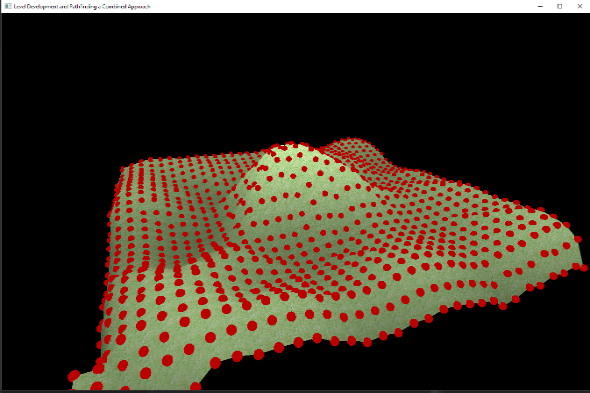
\includegraphics[width=0.5\textwidth]{images/nodes}
	\caption{The node placement when drawn on to the terrain} \label{node}
\end{figure}

\subsection{Path finding implementation}
To allow comparison between different path finding techniques we will implement both Dijkstra's algorithm and A-star when a path is found the nodes that make up the path will change from red \ref{node} to green.  

\subsection{Combining the terrain and path-finding metric}
When it comes to the combination of measurements gathered by the project our first concern is what exactly we are measuring which for the path-finding will be the distance of path from start to finish and the time taken to build a path across the terrain.\\\\To measure the quality of terrain we will look at the standard deviation of the normals and time taken to generate a suitable terrain now to combine these timing measurements is fine as they will be on the same scale.\\\\ There is an issue when deciding how we measure the distance of a path against the standard deviation of the normals on the terrain as these will be scaled differently now there are a few options here firstly we could take lots of path-finding measurements and by working out how much difference there is between these we could establish a scale that would be able to integrate with the standard deviation of the terrain.      


\subsection{Additional Information / Knowledge Required}
To implement the project a solid knowledge of a graphical programming language such as openGL or DirectX is required also perfomance based GPGPU programming API's  such as OpenCL or Nvidia's CUDA could be useful for optimising the project.

The artificial intelligence aspects of the project will require knowledge of various path-finding techniques and also an understanding of machine based learning would be beneficial to allow training of the system for analysis of the terrain and path-finding metric.   
\subsection{Experimental plan}
To determine how well the project works in terms of creating a combined metric for terrain generation and path-finding the following experiments will be run.

\subsubsection{Experiment 1}
For this experiment the aim is to gather the results of both path-finding techniques over a single terrain generated using one type of noise this will allow verification of the path finding techniques and leading on to the integration of a combined metric. 

\subsubsection{Experiment 2}
This experiment will use different instances of terrain generated using various types of noise and both path-finding techniques this will allow testing of the combined metric and show that the project can be utilised in a variety of scenarios.

\subsubsection{After experiment 2} 
As experiment two concludes this will show how the project meets with the aims laid out above \ref{Aims} following on from here the main focus will be to increase the run time performance of the project and to generalise the implementation to increase the area's in which the project can be applied. 

\section{Testing and results}
This table shows the testing carried out from  beginning of implementation it contains reasoning for the tests carried out and the results that were gathered.\\
\begin{tabular}{|p{0.8cm}|p{2cm}|p{5cm}|p{1.4cm}|p{2cm}|}
\hline
Test Id & Test Name & Test Rationale & results & Retesting result (if modified) \\
\hline
1 & Height-map generation and loading & This is the first chosen level generation technique used within the project & pass & n/a\\
\hline
2 & Storage and rendering of height-map & This is necessary to test to allow continued use of the height-map technique & pass & n/a\\
\hline
3 & Height-map performance & This is needed to establish the viability of the height-map method for the project & pass & n/a\\ 
\hline
4 & Other level generation techniques & This could be required if the height-map approach has issues or is not viable due to low performance & pass & may be revisited as additional functionality\\
\hline
5 & Node placement and rendering & This will allow for visualisation of the data for testing and the nodes are required for the path finder & pass & n/a\\ 
\hline
6 & Calculating the distance between all nodes on the generated terrain  & This is required for the path finding algorithm & pass & n/a\\
\hline
7 & Implementation of Dijkstra and A-star path-finding techniques &This will allow for a path to be built through the terrain & ongoing & n/a\\
\hline   
\end{tabular}
\newpage
\section{Conclusions}


\section{Bibliography}
\bibliographystyle{apalike}
\bibliography{Literature-Review/Literature}

\newpage
\begin{appendices}
\section{Project Overview}


% Neil Notman's Hons Project

% Notes:

\pagestyle{fancy}

\lhead{Neil Notman}
\rhead{40124066}
\lfoot{Games Development BSc (Hons)}
\cfoot{}
\rfoot{\thepage}
\title{Procedural level generation and dynamic pathfinding a combined approach}
\author{Initial Project Overview\\Neil Notman\\40124066}
\providecommand{\keywords}[1]{\textbf{Keywords---} #1}
\date{}

\sloppy



\renewenvironment{abstract}
  {\small\quotation
  {\bfseries\noindent{\large\abstractname\\\noindent{}}}}
  {\endquotation}


\setlength\parindent{0cm}


\keywords{Level-Generation,Path-Finding,Algorithm,Optimisation}

\subsection{Overview of  Project Content and Milestones}
This project will include research into current practices used in industry for path-finding and level generation with the emphasis being performance based compared against realism. The main milestone for this stage will be coming across a method to integrate both level generation and path-finding into an algorithm which will be carried forward to the development stage.\\

Development of an application which will utilise both level generation and path-finding either by the modification and optimisation of existing approaches or the creation of a new algorithm. The application will allow the user to create various sizes of level and the application will then give a visual representation of both the level and path that has been built.\\

The application will then be optimised and tested against some of the methods researched with the aim to show that a combined approach may achieve better results in a similar or faster run time with the paths created being checked for mistakes or inconsistencies based on various sanity checks (no path nodes on areas that should not be traversable such as extreme slopes or dips in the level).\\

Creation of a report that contains all project information and related work with a detailed analysis and testing of the approach used to provide an evaluation of the solution using performance figures to accurately examine the viability of this approach in comparison to the current industry standards and draw a conclusion over the project as a whole.\\

For a more detailed look at the time-line for this project please refer to Figure \ref{gantt}\\

\subsection{The Main Deliverables}
\begin{itemize}
\item A application that will allow the user to create various sizes of level and will give a visual output of the level and path built with a focus on the optimisation techniques used to integrate level generation and path finding.\\
\item A detailed report containing an analysis on the approach taken and a comparison between the solution and other methods used currently using figures from both to evaluate the effectiveness and viability of the approach used.\\
\item Test logs of the finished application and an industry standard practice to allow for an unbiased comparison to be made based on results obtained from these tests when documenting the project.
\end{itemize}

\subsection{Target audience for the deliverables}
The deliverables of this project may be of interest to people involved with both level generation and path finding in the games development industry. Researchers involved in this field may find the report and comparison of techniques used to be of interest. Other people may find this project helpful with regards to optimisation techniques. The main aim of the project  is to show the performance of a combined approach to level generation and path-finding and an evaluation of the quality of paths built. 

\subsection{The work to be undertaken}
\begin{itemize}
\item Research into current industry practices for level generation and path finding to allow for visualization of a solution to combine these algorithms.\\
\item Development of the application and chosen approach with a focus on performance while maintaining a level of realism.\\
\item Optimisation of the developed solution and gathering of test data from the solution and an industry approach.\\
\item Creation of a report detailing the approach taken to implementing the project and providing an evaluation between the solution compared to industry practices.  
\end{itemize}
There is a diagram showing expected steps of execution within the application shown at Figure \ref{block}

\subsection{Knowledge and skills required}
To be able to complete the project to a high standard I will first need to research the field’s of both level generation and path finding as a solid knowledge will be needed to create a combined approach. In terms of development further research into optimisation techniques for C++ in Visual Studio will allow for a more polished and better performing solution also as a level of realism will be maintained experience with graphic programming would also benefit the project.  

\subsection{Information sources that provide a context for the project}
The video available at \cite{levels1} gives a few very basic examples of levels that can be generated and also details some methods to define areas within a level(slopes,walls,and others) this definition of areas within a level could be used for testing the path finding within the project and may give a basic concept on how to generate content within the level produced in relation with the project.\\

The paper\cite{paths1} analyses various path-finding algorithms however the purpose of their project was to look at an alternative approach to the A* path finding algorithm.  Use of concepts such as map abstraction could be of interest to this project as it would allow a way to break the level into chunks which can then be processed individually by a path finding algorithm.\\

The textbook for level generation \cite{levels2} Provides extensive research into procedurally generated content in games from grid based levels to full landscapes there are multiple approaches detailed within the textbook that can provide a basis to generate a level within the project.\\

\textbf{Previous honours projects to note}\newline
This paper\cite{honours} analyses various path finding algorithms and discusses at optimisation options this will be the inspiration for optimising the project and will give a wide variety of path finding algorithms to research going forward.\\

For a timeline of research into path finding algorithms please refer to Figure \ref{timeline}

\subsection{The importance of the project}
This project is important as it will seek to integrate level generation and path finding which could allow for faster loading times in games while reducing the storage space taken by a game. When comparing the difference between developed solution and current industry practices - if the solution proves to be better in terms of performance and the quality of the path built is of a suitable standard for the complexity of the level that is generated.   

\subsection{The key challenges to be overcome}
\begin{itemize}
\item  Research of a variety of level generation and path-finding techniques to gain knowledge and propose a viable solution for development.\\
\item Development of  an application that will use the envisioned solution and give a visual output to the user of both level and path built.\\
\item Research into a way of determining the quality of path finding and level generation techniques.\\
\item Writing of a detailed report that will clearly explain the solution chosen and give a view into past work done within this field then the report will provide an unbiased comparison between the approach and current industry practices to evaluate the project in terms of the quality the path built when compared to the complexity of the level generated.
\end{itemize}

\begin{figure}[ht!]
	\begin{tabular}{ |p{5cm}|p{3.5cm}|p{0.8cm}|}
	\hline
            Creator & Method & Year \\
             \hline
            Dijkstra \cite{dijkstra} & Graph searching & 1959 \\
            \hline
            Goodchild \cite{goodchild} & Orthagonal and diagonal movement & 1977\\
            \hline
            Huber and Church \cite{huber} & analysis of neighboring cells & 1985\\
            \hline
            Eastman \cite{eastman} & Pushbroom procedure & 1989\\
            \hline
            Lombard and Church \cite{lombard} & GSP(Gateway-shortest-path) & 1993\\
            \hline
            Mcilhagga \cite{mcilhagga} & Fixed cost distance & 1997\\
            \hline
            Andrea Califano \cite{califano} & Splash algorithm & 2000\\ 
            \hline
\end{tabular} 
	\caption{A time-line of path finding algorithms}	 \label{timeline} \cite{Time}
\end{figure}

\begin{landscape}
\begin{figure}[ht!]
	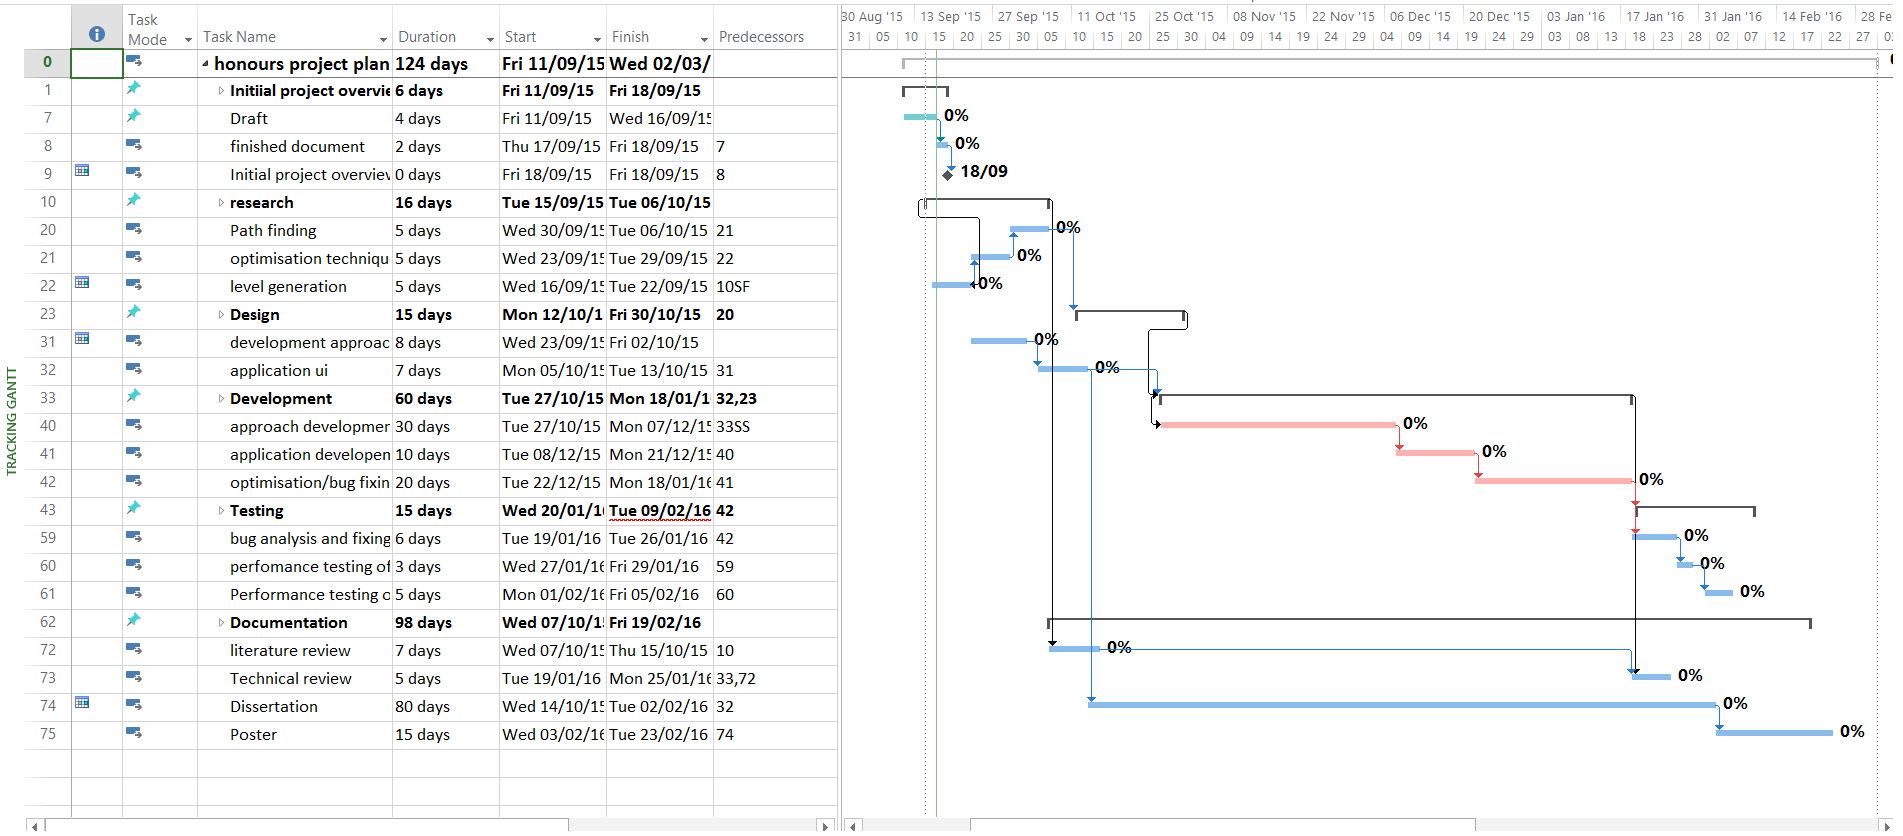
\includegraphics[width=1.5\textwidth]{images/project-plan}
	\caption{An image of the project gantt chart	 \label{gantt}}
\end{figure}
\end{landscape}



\begin{figure}[ht!]
	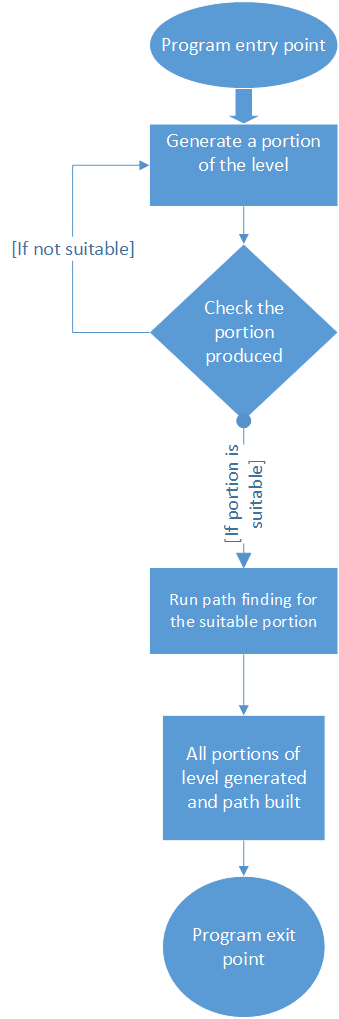
\includegraphics[width=1.0\textwidth, height =1.4\textwidth]{images/block-diagram}
	\caption{This shows how the program will execute	\label{block}}
\end{figure}






\newpage
\begin{landscape}
\begin{figure}[ht!]
	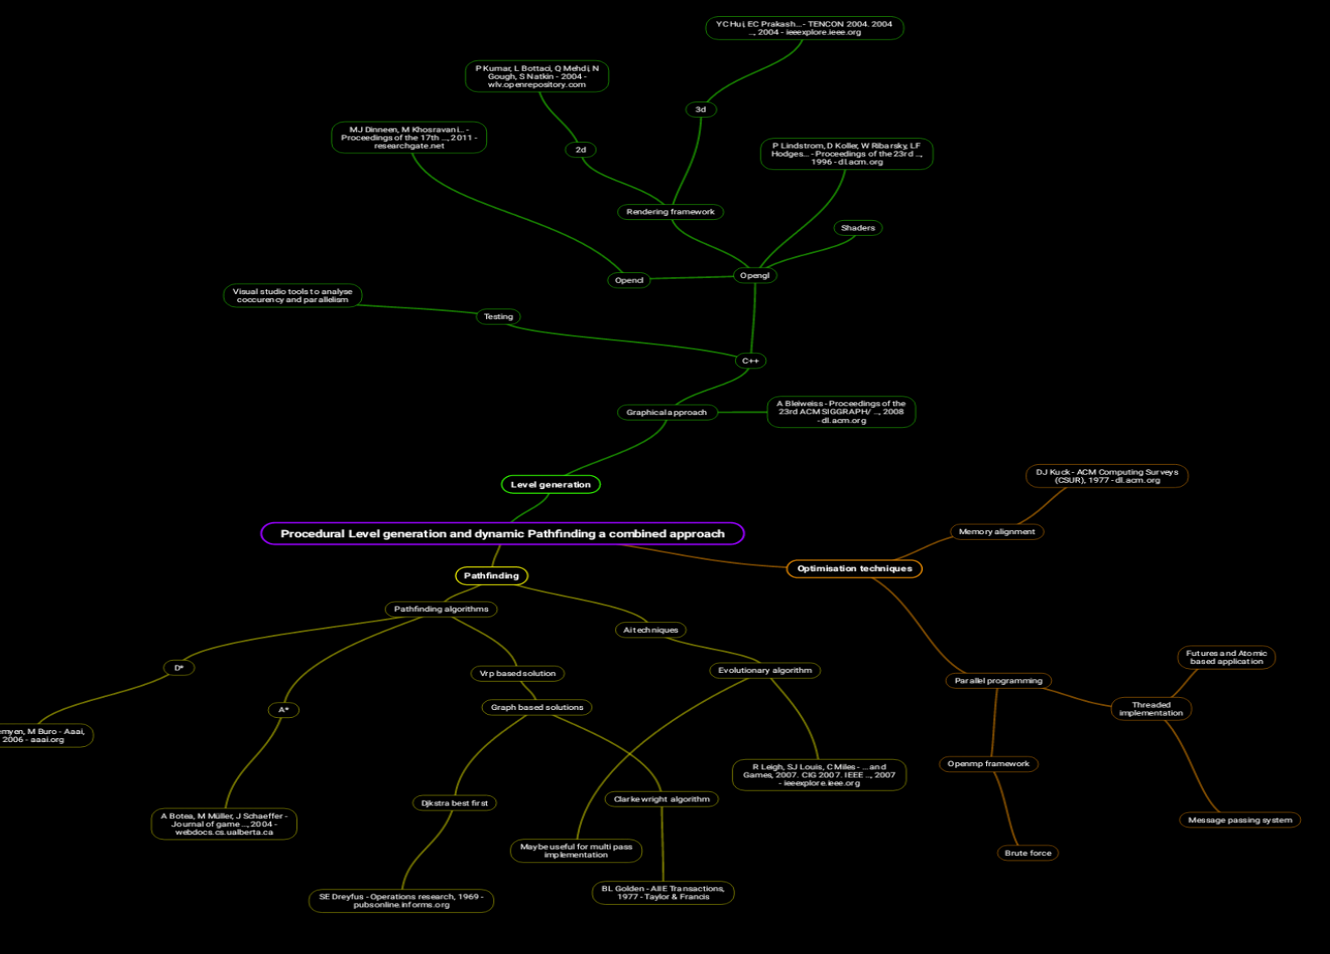
\includegraphics[width=1.4\textwidth, height =1.0\textwidth]{images/Honours-Mind-Map}
	\caption{This is a mind map covering the scope of the project	\label{mind}}
\end{figure}
\end{landscape}
\newpage
\section{Diary Sheets and project management}
\subsection{Week 2 and before}
This was the point where a supervisor for the project was established and formal meetings were begun from week 3.

\subsection{Meeting 1 22/9/15 Week 3}

\textbf{Objectives}\\
update literature/background\\
Polish IPO for submission\\
Block diagram\\\\\textbf{Progress}\\
First draft of IPO and Project plan\\
First meeting\\\\\textbf{Comments}\\
On Track/looking good


\subsection{Meeting 2 29/9/15 Week 4}

\textbf{Objectives}\\
start drafting literature review\\
Mind map\\
Add keywords\\
setup version control with basic renderer\\
Comparison grid\\
\\\\\textbf{Progress}\\
IPO handed in\\
Collecting papers for research\\
Setup blog\\\\\textbf{Comments}\\
On Track


\subsection{Meeting 3 6/10/15 Week 5}

\textbf{Objectives}\\
Thesis template\\
Add main bib file\\
Screen-shots from implementation\\
Add mind map\\
Write introduction\\
Comparison grid\\
\\\\\textbf{Progress}\\
Skeleton Framework\\
Continued Collecting papers for research\\
Added keywords to IPO\\\\\textbf{Comments}\\
Starting to slow down


\subsection{Meeting 4 13/10/15 Week 6}

\textbf{Objectives}\\
Screenshots\\
Add mind map and comparison grid to thesis\\
Fix and complete level generation implementation\\
Draft lit review\\
Write introduction\\
Blog updates\\
Print and bring thesis to next meeting \\
\\\\\textbf{Progress}\\
Height-map generation code implemented\\
Continued Collecting papers for research\\
Drafted thesis and started introduction\\\\\textbf{Comments}\\
Need to improve time management\\
On track-good work

\subsection{Meeting 5/Group Thesis Review 20/10/15 Week 7}

\textbf{Feedback}\\
Report looking good so far minor changes to be made to already completed sections.\\
\\\\\textbf{Progress}\\
Mind map finished and added to thesis.\\
Loading of height-map code fixed. 

\subsection{Meeting 6 27/10/15 Week 8}
Meeting was missed however general discussion was had with supervisor during the week to state goals for this week and record progress informally. 

\subsection{Meeting 6 3/11/15 Week 9}

\textbf{Objectives}\\
Update thesis\\
Look at commercial packages for comparison\\
Implementation work (Test cases)\\
Print and bring thesis to next meeting \\
\\\\\textbf{Progress}\\
Numerical experimentation for level generation\\
Started writing implementation methodology\\
almost finished lit review(Draft version)\\\\\textbf{Comments}\\
Coursework week(busy)\\
Second marker meeting next week

\subsection{Meeting 7 10/11/15 Week 10}

\textbf{Objectives}\\
Update thesis\\
Fix rendering\\
Implementation work (Test cases)\\
Blog/Website updates
Print and bring thesis to next meeting \\
\\\\\textbf{Progress}\\
Started to fix development issues(rendering)\\
Thesis Work\\
Re-done blog/website (more structured)
\\\\\textbf{Comments}\\
Review thesis progress next week\\
Week 10-Second marker meeting organisation  

\subsection{Meeting 8 17/11/15 Week 11}
Second marker meeting.\\\\
\textbf{Feedback}
Following the meeting it was agreed that the project would be based around the creation of a testing mechanism instead of being solely performance based the thesis work to this point was said to be under what was expected however as the project aims shifted this allowed less changes to be made overall there was also guidance on existing projects within the university.


\subsection{Meetings up to 21/3/16}
There has been a lack of formal communication with weekly updates being discussed at any point where we happened to meet however there has been no meetings recently this is due to the absence of my supervisor.    

\subsection{Meeting 9 21/3/17}
\section{Second Formal Review Output}
%Insert a copy of the project review form you were given at the end of the review by the second marker

\section{Appendix 4 and following}
%insert content here and for each of the other appendices, the title may be just on a page by itself, the pages of the appendices are not numbered, unless an included document such as a user manual or design document is itself pager numbered.
\end{appendices}

\end{document}
